% Beamer Presentation for dpol_breakup Experiment Optimization
% Date: November 26, 2025
% Author: Tian

\documentclass[aspectratio=169]{beamer}
\usetheme{Madrid}
\usecolortheme{default}

% Packages
\usepackage{graphicx}
\usepackage{amsmath}
\usepackage{amssymb}
\usepackage{booktabs}
\usepackage{listings}
\usepackage{xcolor}
\usepackage{hyperref}
\usepackage{tikz}
\usetikzlibrary{shapes,arrows,positioning}

% Code listing settings
\lstset{
  basicstyle=\ttfamily\footnotesize,
  breaklines=true,
  frame=single,
  numbers=left,
  numberstyle=\tiny\color{gray},
}

% Title page information
\title[dpol\_breakup Optimization]{Progress Report: Optimization of dpol\_breakup Experiment Configuration}
\subtitle{Simulation Framework and Configuration Study}
\author[Tian]{Tian}
\institute[]{SAMURAI Collaboration}
\date{November 26, 2025}

% Footer customization
\setbeamertemplate{footline}[frame number]

\begin{document}

% Title slide
\begin{frame}
\titlepage
\end{frame}

% Table of contents
\begin{frame}{Outline}
\tableofcontents
\end{frame}

% ============================================
% Section 1: Objectives
% ============================================
\section{Research Objectives}

\begin{frame}{Research Objectives}
\begin{block}{Primary Goal}
Determine the optimal experimental configuration for the \texttt{dpol\_breakup} experiment by evaluating detection efficiency and reconstruction accuracy.
\end{block}

\vspace{0.5cm}

\textbf{Key Questions:}
\begin{enumerate}
\item What is the optimal target position for different magnetic field strengths?
\item How does the beam deflection angle affect detection efficiency?
\item What momentum resolution can we achieve with the current PDC setup?
\item How can we improve reconstruction speed and accuracy?
\end{enumerate}
\end{frame}

% ============================================
% Section 2: System Architecture
% ============================================
\section{System Architecture}

\begin{frame}{Complete Simulation Framework}
\begin{center}
\scalebox{0.75}{
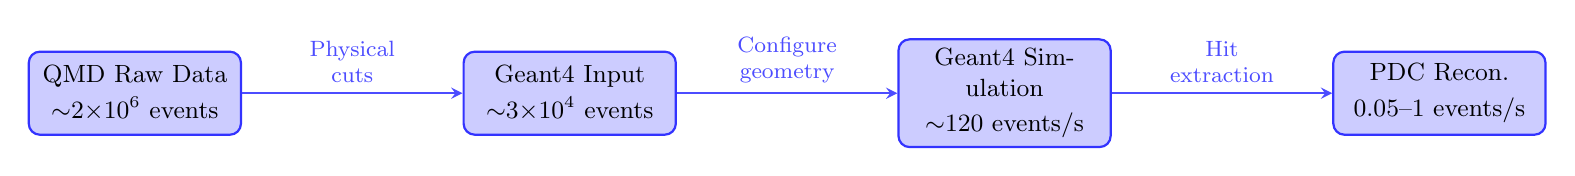
\begin{tikzpicture}[
  node distance=2.8cm,
  block/.style={rectangle, draw=blue!80, fill=blue!20, thick,
    text width=7em, text centered, rounded corners, minimum height=3em,
    font=\small},
  arrow/.style={->, thick, >=stealth, blue!70}
]

% Nodes - left to right
\node [block] (qmd) {QMD Raw Data\\[0.2em]$\sim$2$\times$10$^6$ events};
\node [block, right=of qmd] (g4input) {Geant4 Input\\[0.2em]$\sim$3$\times$10$^4$ events};
\node [block, right=of g4input] (g4sim) {Geant4 Simulation\\[0.2em]$\sim$120 events/s};
\node [block, right=of g4sim] (pdc) {PDC Recon.\\[0.2em]0.05--1 events/s};

% Arrows with labels on top
\draw [arrow] (qmd) -- node[above, align=center, font=\footnotesize] {Physical\\cuts} (g4input);
\draw [arrow] (g4input) -- node[above, align=center, font=\footnotesize] {Configure\\geometry} (g4sim);
\draw [arrow] (g4sim) -- node[above, align=center, font=\footnotesize] {Hit\\extraction} (pdc);

\end{tikzpicture}
}
\end{center}
\end{frame}

\begin{frame}{Framework Components}
\begin{itemize}
\item \textbf{Scripts}: QMD data transformation, cutting, sampling, reconstruction analysis
\item \textbf{Visualization}: 3D event display and batch processing
\item \textbf{Status}: Core framework operational and ready for optimization
\end{itemize}

\vspace{0.5cm}

\begin{alertblock}{Current Bottleneck}
PDC reconstruction speed: 0.05-1 events/s (target: $>$10 events/s)
\end{alertblock}
\end{frame}

% ============================================
% Section 3: Performance Benchmarks
% ============================================
\section{Performance Benchmarks}

\begin{frame}{Performance Status}
\begin{columns}
\column{0.5\textwidth}
\textbf{Current Performance:}
\begin{itemize}
\item Geant4 Simulation: \textcolor{green}{$\sim$120 events/s}
\item PDC Reconstruction: \textcolor{red}{0.05-1 events/s}
\item Issues: Systematic momentum bias
\end{itemize}

\column{0.5\textwidth}
\textbf{Target Performance:}
\begin{itemize}
\item Reconstruction: $>$10 events/s
\item Momentum resolution: ?? 
\item Detection efficiency: ?? (for config target position)
\end{itemize}
\end{columns}

\vspace{1cm}

\begin{block}{Performance Challenges}
\begin{itemize}
\item Speed bottleneck in track fitting
\item TMinuit convergence issues
\item Systematic bias for certain momentum ranges
\end{itemize}
\end{block}
\end{frame}

% ============================================
% Section 4: QMD Data Processing
% ============================================
\section{QMD Data Processing}

\begin{frame}{Data Processing Strategy}
\textbf{Challenge:} Massive data volume ($\sim$2$\times$10$^6$ events per configuration)

\vspace{0.5cm}

\textbf{Solution:} Apply physical cuts to focus on region of interest

\begin{table}
\centering
\small
\begin{tabular}{lcc}
\toprule
\textbf{Selection Stage} & \textbf{Conditions} & \textbf{Event Count} \\
\midrule
No Cut & - & $2 \times 10^6$ \\
Momentum Cut & $|p_{y,p} - p_{y,n}| < 150$ MeV/c & $5 \times 10^5$ \\
 & $(p_{x,p} + p_{x,n}) < 200$ MeV/c & \\
Angular Cut & $|\pi - |\phi_{rot}|| < 0.2$ rad & $3 \times 10^4$ \\
\bottomrule
\end{tabular}
\end{table}

\vspace{0.3cm}
\textbf{Result:} 98.5\% data reduction while preserving physics of interest
\end{frame}

\begin{frame}{QMD Data Flow}
\begin{center}
\includegraphics[width=0.75\textwidth]{assets_20251126_en/image-4.png}
\end{center}
\end{frame}

% ============================================
% Section 5: Geant4 Simulation
% ============================================
\section{Geant4 Simulation Results}

\begin{frame}{Current Configuration}
\begin{itemize}
\item \textbf{Target position:} Based on 5$^{\circ}$ beam deflection in 1.2 T field
\item \textbf{Magnetic field:} 1.2 Tesla
\item \textbf{Detector geometry:} PDC1, PDC2, NEBULA array
% \item \textbf{Beam energy:} 190 MeV/nucleon (deuteron)
\end{itemize}

\vspace{0.5cm}

\textbf{Planned Parameter Scan:}
\begin{itemize}
\item Magnetic field: 1.2, 1.4, 1.6 Tesla (for pdc acceptance and resolution)
\item Beam deflection angles: 0 (outside chamber), 5 degrees(inside), other angles
\item Target positions: related to B and beam angle.
\item PDC position (related to above all)
\end{itemize}
\end{frame}

\begin{frame}{Simulation Visualization}

5deg 1.2T Configuration

\begin{columns}
\column{0.5\textwidth}
\begin{center}
\includegraphics[width=\textwidth]{assets_20251126_en/image.png}
\small{5000 accumulated events}
\end{center}

\column{0.5\textwidth}
\begin{center}
\includegraphics[width=\textwidth]{assets_20251126_en/image-1.png}
\small{Detection efficiency}
\end{center}
\end{columns}
\end{frame}

\begin{frame}{Comparison with Reference Data}
\begin{columns}
\column{0.5\textwidth}
\begin{center}
\includegraphics[width=\textwidth]{assets_20251126_en/image-2.png}
\small{Reference from paper}
\end{center}
\column{0.5\textwidth}
\begin{center}
\includegraphics[width=0.8\textwidth]{assets_20251126_en/image-3.png}
\small{Experimental setup}
\end{center}
\end{columns}

\vspace{0.3cm}
\textbf{Conclusion:} Our results are consistent with published references
\end{frame}

% ============================================
% Section 6: PDC Reconstruction
% ============================================
\section{PDC Reconstruction}

\begin{frame}{Reconstruction Methodology}
\textbf{Principle:} PDC determines particle \textit{direction}; optimize \textit{momentum magnitude} by minimizing distance to target

\vspace{0.5cm}

\textbf{Implemented Algorithms:}
\begin{enumerate}
\item \textbf{Grid Search}
\begin{itemize}
\item[$+$] Robust, finds global minimum
\item[$-$] Computationally expensive
\end{itemize}

\item \textbf{Gradient Descent}
\begin{itemize}
\item[$-$] slow convergence (now situation)
\item[$-$] Sensitive to local minima and noise (in this no local minima)
\end{itemize}

\item \textbf{TMinuit (ROOT)} \textcolor{blue}{$\leftarrow$ Current primary method}
\begin{itemize}
\item Uses MIGRAD/SIMPLEX algorithms
\item Fallback strategy if MIGRAD fails
\end{itemize}
\end{enumerate}
\end{frame}

\begin{frame}{Current Challenges}
\begin{block}{Issue 1: Reconstruction Quality}
Inconsistent performance - subset shows poor results
\end{block}

\begin{block}{Issue 2: Momentum Bias}
Double-peak structure in residuals ($\Delta p = p_{reco} - p_{true}$):
\begin{itemize}
\item Peak 1: $\sim$0 MeV/c (correct reconstruction)
\item Peak 2: $\sim$-200 MeV/c (systematic underestimation)
\end{itemize}
\end{block}

\begin{block}{Issue 3: Speed Bottleneck}
Reconstruction: 1-20 seconds per event (too slow for production)
\end{block}
\end{frame}

\begin{frame}{Reconstruction Results (1/3)}
\begin{center}
\includegraphics[width=0.9\textwidth]{assets_20251126_en/image-5.png}\\
\small{Neutron momentum: Reco vs Input}
\end{center}
\end{frame}

\begin{frame}{Reconstruction Results (2/3)}
\begin{center}
\includegraphics[width=0.7\textwidth]{assets_20251126_en/image-6.png}\\
\small{TMinuit optimization steps}
\end{center}
\end{frame}

\begin{frame}{Reconstruction Results (3/3)}
\begin{columns}
\column{0.5\textwidth}
\begin{center}
\includegraphics[width=\textwidth]{assets_20251126_en/image-7.png}\\
\small{3D event display}
\end{center}

\column{0.5\textwidth}
\begin{center}
\includegraphics[width=\textwidth]{assets_20251126_en/image-8.png}\\
\small{Zoomed view -- track back-propagation}
\end{center}
\end{columns}
\end{frame}

\begin{frame}[fragile]{Example Case: Convergence Issues}
\textbf{Input:} Proton, $|p| = 629.0$ MeV/c

\begin{lstlisting}[language=bash, basicstyle=\ttfamily\tiny, escapechar=!]
Initial momentum guess: 800 MeV/c

MIGRAD failed with error code: 4
Trying SIMPLEX algorithm...

TMinuit optimization completed:
  Best momentum: 618.13 +/- 2849.91 MeV/c  !\textcolor{red}{$\leftarrow$ Huge uncertainty!}!
  Final distance: 4.79785 mm
  Convergence status: 1 (3=converged)
  EDM (estimated distance to minimum): 2.84217e-14
\end{lstlisting}

\vspace{0.3cm}
\textbf{Analysis:}
\begin{itemize}
\item Result (618 MeV/c) close to true value (629 MeV/c)
\item But uncertainty ($\pm$2850 MeV/c) indicates convergence problems
\item Likely stuck in local minimum, not global minimum
\end{itemize}
\end{frame}

\begin{frame}{Momentum Correlation \& Residuals}
\begin{columns}
\column{0.5\textwidth}
\begin{center}
\includegraphics[width=\textwidth]{assets_20251126_en/image-10.png}
\small{2D correlation: True vs Reconstructed}
\end{center}

\column{0.5\textwidth}
\begin{center}
\includegraphics[width=\textwidth]{assets_20251126_en/image-9.png}
\small{Residual distribution - double peak}
\end{center}
\end{columns}
\end{frame}

% ============================================
% Section 7: Technical Details
% ============================================
\section{Technical Implementation}

\begin{frame}{Core Algorithms}
\textbf{1. PDC Hit Reconstruction}
\begin{itemize}
\item Center-of-mass weighted energy deposition method
\item Process U and V layers independently
\item Gaussian smearing: $\sigma \approx 0.5$ mm
\item Transform coordinates for spectrometer rotation
\end{itemize}

\vspace{0.5cm}

\textbf{2. Runge-Kutta Integration (4th order)}
\begin{itemize}
\item Solve particle motion in magnetic fields
\item Relativistic kinematics: $E = \sqrt{p^2 + m^2}$
\item Lorentz force: $\frac{dp}{dt} = q(v \times B)$
\item Step size: 1 mm (trade-off: accuracy vs speed)
\end{itemize}
\end{frame}

\begin{frame}{Momentum Optimization \& Neutron Reconstruction}
\textbf{3. TMinuit Objective Function}
\begin{equation}
\chi^2 = \sqrt{(x_{track} - x_{target})^2 + (y_{track} - y_{target})^2 + (z_{track} - z_{target})^2}
\end{equation}

\vspace{0.3cm}

\textbf{4. NEBULA Neutron Reconstruction}
\begin{itemize}
\item Time-of-Flight (TOF) based - no magnetic field effect
\item Energy-weighted position clustering
\item Time window: 10 ns
\item Energy threshold: 1 MeV
\end{itemize}

Physics formulas:
\begin{align*}
\beta &= \frac{d_{flight} / t_{flight}}{c}, \quad
\gamma = \frac{1}{\sqrt{1-\beta^2}}\\
KE &= (\gamma - 1) \times m_n, \quad
p = \gamma m_n \beta c
\end{align*}
\end{frame}

% ============================================
% Section 8: Optimization Strategy
% ============================================
\section{Optimization Strategy}

\begin{frame}{Six-Point Optimization Plan}
\begin{enumerate}
\item \textbf{Algorithm Optimization}
\begin{itemize}
\item Adjust Runge-Kutta step size (1 mm $\rightarrow$ 2-5 mm)
\item Tune magnetic field integration precision
\end{itemize}

\item \textbf{Batch Processing}
\begin{itemize}
\item Memory-efficient analysis
\item Discard unnecessary track objects during I/O
\end{itemize}

\item \textbf{Parallel Computing}
\begin{itemize}
\item Multi-threading for simultaneous event processing
\end{itemize}

\item \textbf{I/O Optimization}
\begin{itemize}
\item Asynchronous logging to prevent blocking
\end{itemize}

\item \textbf{Smart Initial Guess}
\begin{itemize}
\item Use PDC direction and typical momentum range
\item Improve TMinuit convergence
\end{itemize}

\item \textbf{Adaptive Step Size}
\begin{itemize}
\item RK step depends on B-field strength and curvature
\end{itemize}
\end{enumerate}
\end{frame}

% ============================================
% Section 9: Next Steps
% ============================================
\section{Next Steps \& Summary}

\begin{frame}{Priority Tasks}
\begin{block}{High Priority}
\begin{enumerate}
\item Complete QMD data sampling $\rightarrow$ Generate ROOT files for Geant4
\item Optimize simulation \& reconstruction code for speed
\item Systematic configuration study (B-field, target, beam angle)
\end{enumerate}
\end{block}

\begin{block}{Medium Priority}
\begin{enumerate}
\item Investigate isovector effects in deuteron simulations
\item Evaluate systematic uncertainties
\item Validate against experimental data
\end{enumerate}
\end{block}

\begin{block}{Low Priority}
\begin{enumerate}
\item Complete technical documentation
\item Code refactoring for maintainability
\end{enumerate}
\end{block}
\end{frame}

\begin{frame}{Summary}
\begin{columns}
\column{0.5\textwidth}
\textbf{Achievements:}
\begin{itemize}
\item[$\checkmark$] Complete simulation framework
\item[$\checkmark$] Multiple reconstruction algorithms
\item[$\checkmark$] Identified bottlenecks
\item[$\checkmark$] Baseline benchmarks
\end{itemize}

\column{0.5\textwidth}
\textbf{Current Challenges:}
\begin{itemize}
\item[!] Speed: 0.05-1 Hz $\rightarrow$ need $>$10 Hz
\item[!] Momentum bias (double-peak)
\item[!] Large statistics needed
\end{itemize}
\end{columns}

\vspace{1cm}

\begin{block}{Key Milestones}
\begin{enumerate}
\item Complete QMD sampling for production-scale input
\item Optimize reconstruction to 10 Hz
\item Run systematic configuration scans
\item Validate against experimental data
\end{enumerate}
\end{block}
\end{frame}

% ============================================
% Final slide
% ============================================
\begin{frame}{Thank You}
\begin{center}
{\Large Thank you for your attention!}

\vspace{1cm}

\textbf{Questions \& Discussion}

\vspace{1cm}

\small
\textbf{Contact:}\\
Tian (\texttt{tbt23@mails.tsinghua.edu.cn})\\
Repository: \texttt{github.com/tianbaiting/Dpol\_smsimulator}\\
Branch: \texttt{restructure-cmake}
\end{center}
\end{frame}

% Backup slides
\appendix
\section{Backup Slides}

\begin{frame}{Backup: Additional Technical Details}
\textbf{Available for further discussion:}
\begin{itemize}
\item Detailed Runge-Kutta implementation
\item TMinuit configuration parameters
\item Memory profiling results
\item Parallelization strategies
\item Code structure and API documentation
\end{itemize}
\end{frame}

\end{document}
